\documentclass[a4,useAMS,usenatbib,usegraphicx]{mn2e} 
%=========================================================================
\usepackage{amsmath} 
\usepackage{amssymb} 
\usepackage {graphicx}
\usepackage[dvips]{epsfig}
\usepackage{epsfig}  
\usepackage{color}
\usepackage[normalem]{ulem}
\usepackage{hyperref}
\usepackage{caption}
%Non reposionated tables
\usepackage{float}
\restylefloat{table}
%Multiple columns support for tables
\usepackage{array}
\usepackage{booktabs}
\setlength{\heavyrulewidth}{1.5pt}
\setlength{\abovetopsep}{4pt}


%=========================================================================
%		INTERNAL MACROS
%=========================================================================
\def\be{\begin{equation}}
\def\ee{\end{equation}}
\def\ba{\begin{eqnarray}}
\def\ea{\end{eqnarray}}

% To highlight comments 
\definecolor{red}{rgb}{1,0.0,0.0}
\newcommand{\red}{\color{red}}
\definecolor{darkgreen}{rgb}{0.0,0.5,0.0}
\newcommand{\SRK}[1]{\textcolor{darkgreen}{\bf SRK: \textit{#1}}}
\newcommand{\SRKED}[1]{\textcolor{darkgreen}{\bf #1}}
\newcommand{\before}[1]{\textcolor{red}{ #1}}
\newcommand{\after}[1]{\textcolor{darkgreen}{ #1}}

\newcommand{\tol}{Tololo 1214-277}
\newcommand{\lya}{Ly$\alpha$}
\newcommand{\hb}{H$\beta$}
\newcommand{\ha}{H$\alpha$}
\newcommand{\oiii}{[OIII]}
\newcommand{\oii}{[OII]}
\newcommand{\nii}{[NII]}
\newcommand{\esca}{erg cm$^{-2}$ s$^{-1}$ \AA$^{-1}$}
\newcommand{\esc}{erg cm$^{-2}$ s$^{-1}$}
\newcommand{\es}{erg s$^{-1}$}
\newcommand{\esa}{erg s$^{-1}$}
\newcommand{\kms}{km s$^{-1}$}
\newcommand{\apj}{ApJ}  
\newcommand{\jcap}{JCAP}  
\newcommand{\apjs}{ApJS}  
\newcommand{\pasa}{PASA}  
\newcommand{\apjl}{ApJL}  
\newcommand{\aj}{AJ}  
\newcommand{\mnras}{MNRAS}  
\newcommand{\mnrassub}{MNRAS accepted}  
\newcommand{\aap}{A\&A}  
\newcommand{\aaps}{A\&AS}  
\newcommand{\araa}{ARA\&A}  
\newcommand{\nat}{Nature}  
\newcommand{\physrep}{PhR}
\newcommand{\pasp}{PASP}    
\newcommand{\pasj}{PASJ}    
\newcommand{\sigmaclump}{$54.3\pm 0.6$ km s$^{-1}$}
\newcommand{\inftyclump}{$54.3\pm 5.1$ km s$^{-1}$}
\newcommand{\probaclump}{$0.96\pm 0.01$}
\def\simgt{\lower.5ex\hbox{\gtsima}}
\def\simlt{\lower.5ex\hbox{\ltsima}}

\begin{document}

%=========================================================================
%		FRONT MATTER
%=========================================================================
\title[An atypical \lya\ dwarf galaxy]{
Modelling the gas kinematics of an atypical Lyman alpha emitting compact dwarf galaxy}
\author[J.E. Forero-Romero et al.]
{Jaime E. Forero-Romero $^{1}$ \thanks{je.forero@uniandes.edu.co},
Max Gronke$^2$, 
Maria Camila Remolina-Guti\'errez$^1$,
\newauthor
Nicol\'as Garavito-Camargo$^3$, 
Mark Dijkstra$^2$\\
%%
$^1$ Departamento de F\'isica, Universidad de los Andes, Cra. 1
  No. 18A-10 Edificio Ip, CP 111711, Bogot\'a, Colombia \\
$^2$ Institute of Theoretical Astrophysics, University of Oslo,
Postboks 1029 Blindern, NO-0315 Oslo, Norway.\\
$^3$ Department of Astronomy, University of Arizona, 933 North Cherry
Avenue, Tucson, AZ 85721, USA. 
}

%\vspace*{6pt}\\

%}
\maketitle


\begin{abstract}
  Star-forming Compact Dwarf Galaxies (CDGs) resemble the expected
  pristine conditions of the first galaxies in the Universe and
  are the best systems to test models on primordial
galaxy formation and evolution.    
Here we report on one of such CDGs, \tol, which presents
a broad symmetric \lya\ line emission that had evaded theoretical
interpretation so far. 
In this paper we explain these features by two different kinematic models: 
an interstellar medium composed by outflowing clumps with 
random motions and an homogeneous gaseous sphere undergoing solid body
rotation.
It is the first time that an observed \lya\ spectrum can be explained
assuming either of these kinematic conditions.
We find that both models independently require high velocities
(either a clump velocity dispersion of \sigmaclump\ with outflows of
\inftyclump\ or a bulk rotation of $348^{+75}_{-48}$ km s$^{-1}$)
consistent with a dynamical mass of at 
least a $10^{10}$ M$_{\odot}$, ten times larger than its estimated
baryonic mass.     
We argue that a possible explanation for this excess of
dynamical mass is the presence of a supermassive black hole at the
center of \tol. 
This work suggests the importance of considering multiphase
kinematics and rotation among the possible conditions shaping the
\lya\ spectra of the first galaxies.  
Additionally, if future kinematic maps of \tol\ confirm the 
velocities found by our models, it would provide new
evidence for dwarf galaxies as hosts of supermassive black
holes.  
\end{abstract}

\begin{keywords}
galaxies: dwarf --- galaxies: individual:\tol\ --- radiative transfer --- Methods: numerical 
\end{keywords}


%=========================================================================
%		PAPER CONTENT
%=========================================================================

%*************************************************************************
\section{Introduction}
\label{sec:introduction}





Primordial galaxies have not been detected yet. 
However, dwarf star forming galaxies with a low metallicity content
are seen as templates to understand the early galaxy evolution process. 
Over fifty years ago it was realized that young galaxies could be
detected through a strong \lya\ line emission \citep{PartridgePeebles}.    


This theoretical prediction was only confirmed thirty years later on
distant, relatively young, not primordial, galaxies \citep{1998ApJ...498L..93D}.
Currently Lyman Alpha Emitting (LAE) galaxies are commonly targeted
in surveys. 
The presence of the \lya\ emission line provides confirmation of
the distance to a galaxy while provides clues about the stellar
population and inter-stellar medium conditions regulating the
\lya\ emission.
A careful clustering analysis of LAEs can also yield clues about their link
to dark matter halos
\citep{2004AJ....128.2073H,2007ApJ...671..278G,2007ApJ...668...15K,2008MNRAS.391.1589O,2010MNRAS.409..184P,2013MNRAS.431.1777G,2016ApJ...828....5M}. 

The \lya\ emission line is not exclusive of distant galaxies. 
There are local Universe surveys that target \lya\ emission in nearby
dwarf star forming galaxies.
The study of nearby LAE samples has allowed the study of other
indicators that might be more difficult to obtain for distant galaxies
such as galaxy morphology, dust attenuation, neutral hydrogen contents and
ionization state. See \cite{Hayes15} and references therein for a review.

However, the physical interpretation of \lya\ observations is
not straightforward \citep{LARS,2015ApJ...805...14R}. 
This is due to the resonant nature of the \lya\ line. 
A \lya\ photon follows a diffusion-like process before escaping
the galaxy or being absorbed by dust. 
The resulting line profile becomes sensitive to the dynamical, chemical
and thermal conditions in the interstellar medium. 
There are few analytical tools available to interpret the
emerging \lya\ line
\citep{Harrington73,1991ApJ...370L..85N,LoebRybicki,2006ApJ...645..792T}. 
They are applicable only in cases of highly symmetrical
conditions of the gaseous hydrogen distribution in the galaxy model,
which are hardly met in real astrophysical systems. 
For these reasons the interpretation of \lya\ observations
requires state-of-the-art Monte Carlo radiative transfer simulations.   

\tol\ is a compact star forming dwarf galaxy that presents a
strong \lya\ emission \citep{Thuan97} with two puzzling 
features: the line is symmetric, single peaked and wide around the
line's center.
Usually the \lya\ line has an asymmetric single or double peak. 
These two special features in \tol\ cannot be explained quantitatively
with conventional shell models
\citep{mashesse03,2012ApJ...751...29Y,2015A&A...578A...7V,2015ApJ...812..123G}.   

This kind of profile also raises the question whether some high redshift
LAEs have asymmetric lines because the blue half was truncated by the
intergalactic medium \citep{2007MNRAS.377.1175D}. 
In this case the \lya\ radiation could emerge as a low surface
brightness glow, which may be connected to \lya\ halos, while also
influencing the way LAEs can be used as a probe of reionization
See the review by \cite{2014PASA...31...40D} and the references therein.

Here we show how the \tol's \lya\ profile can be explained
either by  or the recently developed class of complex multiphase models 
\citep{Gronke2016} or by a simple rotation model
\citep{GaravitoCamargo2014}. 
The models we use correspond to simplified geometrical configurations
to allow a deep exploration of parameter space and gain, for the first time,
some physical insight into the \tol's kinematic properties.

We review first the observational characteristics of
\tol, then we summarize the main features in the multiphase and
rotation models to explain how we fit their free parameters 
to the \tol's \lya\ line shape.
We use the results to interpret them in terms of the galaxy's
dynamical mass. 
We close by discussing the physical scenarios opened up by our
results and the additional observational information needed to clarify
the kinematic nature of \tol.


\section{Observations}
\tol's basic observational characteristics are summarized in Table \ref{obstable}.
Its receding velocity is $7785\pm 50$km s$^{-1}$, which translates
into a distance of $106.6$ Mpc (with the Hubble constant $H_{0}$=73
km s$^{-1}$ Mpc$^{-1}$.) 

The observed flux for the \lya\ line is $\sim
8.1\times 10^{-14}$ erg cm$^{-2}$ s$^{-1}$ \citep{Thuan97}
and a Equivalent Width of $70$\AA\ and its H$\beta$ flux is 
$1.62\times 10^{-14}$ erg cm$^{-2}$ s$^{-1}$ \AA${-1}$
\citep{Izotov04} which gives a \lya/H$\beta$ flux ratio of
4.9$\pm$0.1.
The \lya\ flux values correspond to a luminosity of
$L_{Ly\alpha}=2.2\times 10^{42}$ erg s$^{-1}$, which in turn
translates  into a lower bound for the star formation rate of $2.0$
M$_{\odot}$ yr$^{-1}$ after using a standard conversion factor between
luminosity and star formation rate of $9.1\times 10^{-43}$
$L_{Ly\alpha}$ M$_{\odot}$ yr$^{-1}$ \citep{Kennicutt98} without any
correction by extinction.  
Comparing the \lya/H$\beta$ ratio with the theoretical
expectation from case B recombination of $23.3$ \citep{Hummer1987} one
can estimate an escape fraction of $20$\% for \lya\ radiation.

The bolometric UV luminosity is $9.43\pm1.94 \times 10^{8}$
L$_{\odot}$ as measured by GALEX, without any correction by extinction
and following the empirical relation by \cite{Kennicutt98}, this
corresponds to a star formation rate of $0.35\pm 0.05$ M$_{\odot}$
yr$^{-1}$. 
Its metallicity is $\sim Z_{\odot}/24$ as derived from
optical spectroscopy \citep{Izotov04}. 

%The absolute magnitude in the $V$ band translates into a luminosity of
%$8.9\times 10^{8}$ L$_{\odot}$.  
% using http://tomdwelly.com/tools_fluxtolum.php
%


The near-infrared fluxes at $3.6$ $\mu$m and $4.5$ $\mu$m are
$7.71\pm0.55\times 10^{-5}$ Jy and $7.98\pm0.71\times 10^{-5}$ Jy
\citep{2008ApJ...678..804E}.
Using the conversion between fluxes and
stellar mass, $M_{\star} =
10^{5.65} \times F_{3.6}^{2.85} \times F_{4.5}^{-1.85} \times
(D/0.05)^2 M_{\odot}$,  calibrated on the Large Magellanic Cloud 
and  where fluxes are in Jy and $D$ is the luminosity
distance to the source in Mpc, we find $M_{\star} = 1.45\pm0.45\times 10^{8}
M_{\odot}$, with a $30\%$ uncertainty coming from the calibration
process \citep{2012AJ....143..139E}.  

We computed the projected half-light radius to be $R_s=1.5\pm0.1$ kpc 
from the surface brightness profiles reported by \cite{2003A&A...410..481N}. 
Assuming spherical geometry, one can translate this value into a 3D
half-light radius of $r_s=3R_s/2=2.25$ kpc.

There is an upper limit for the  21 cm line integrated flux of $<0.10$
Jy km s$^{-1}$ \citep{pustilnikmartin07}, which translates into a
upper limit for the HI mass of $M<2.65\times 10^{8}$ M$_{\odot}$.  
 



\begin{table}
\begin{center}
\begin{tabular}{lc}\hline
$\alpha$(2000)$^{a}$ & 12h17min17.1s\\
$\delta$(2000)$^{b}$ & -28d02m32s\\
$l$, $b$ (deg) & 294, 34\\
$m_V$ & 17.5\\
  M$_V$ & -17.6\\ 
$v$(km s$^{-1}$) & 7795\\
\lya\ (erg cm$^{-2}$ s$^{-1}$ \AA$^{-1}$)& $8.1\times 10^{-14}$ \\
\lya\ Equivalent Width (\AA) & $70$\\
$21$cm (Jy km s$^{-1}$)& $<0.10$ \\\hline
\end{tabular}
\end{center}
\caption{Basic observational characteristics of \tol\ 
  \citep{Thuan97}\label{obstable}} 
\end{table}



\begin{figure*}
\begin{center}
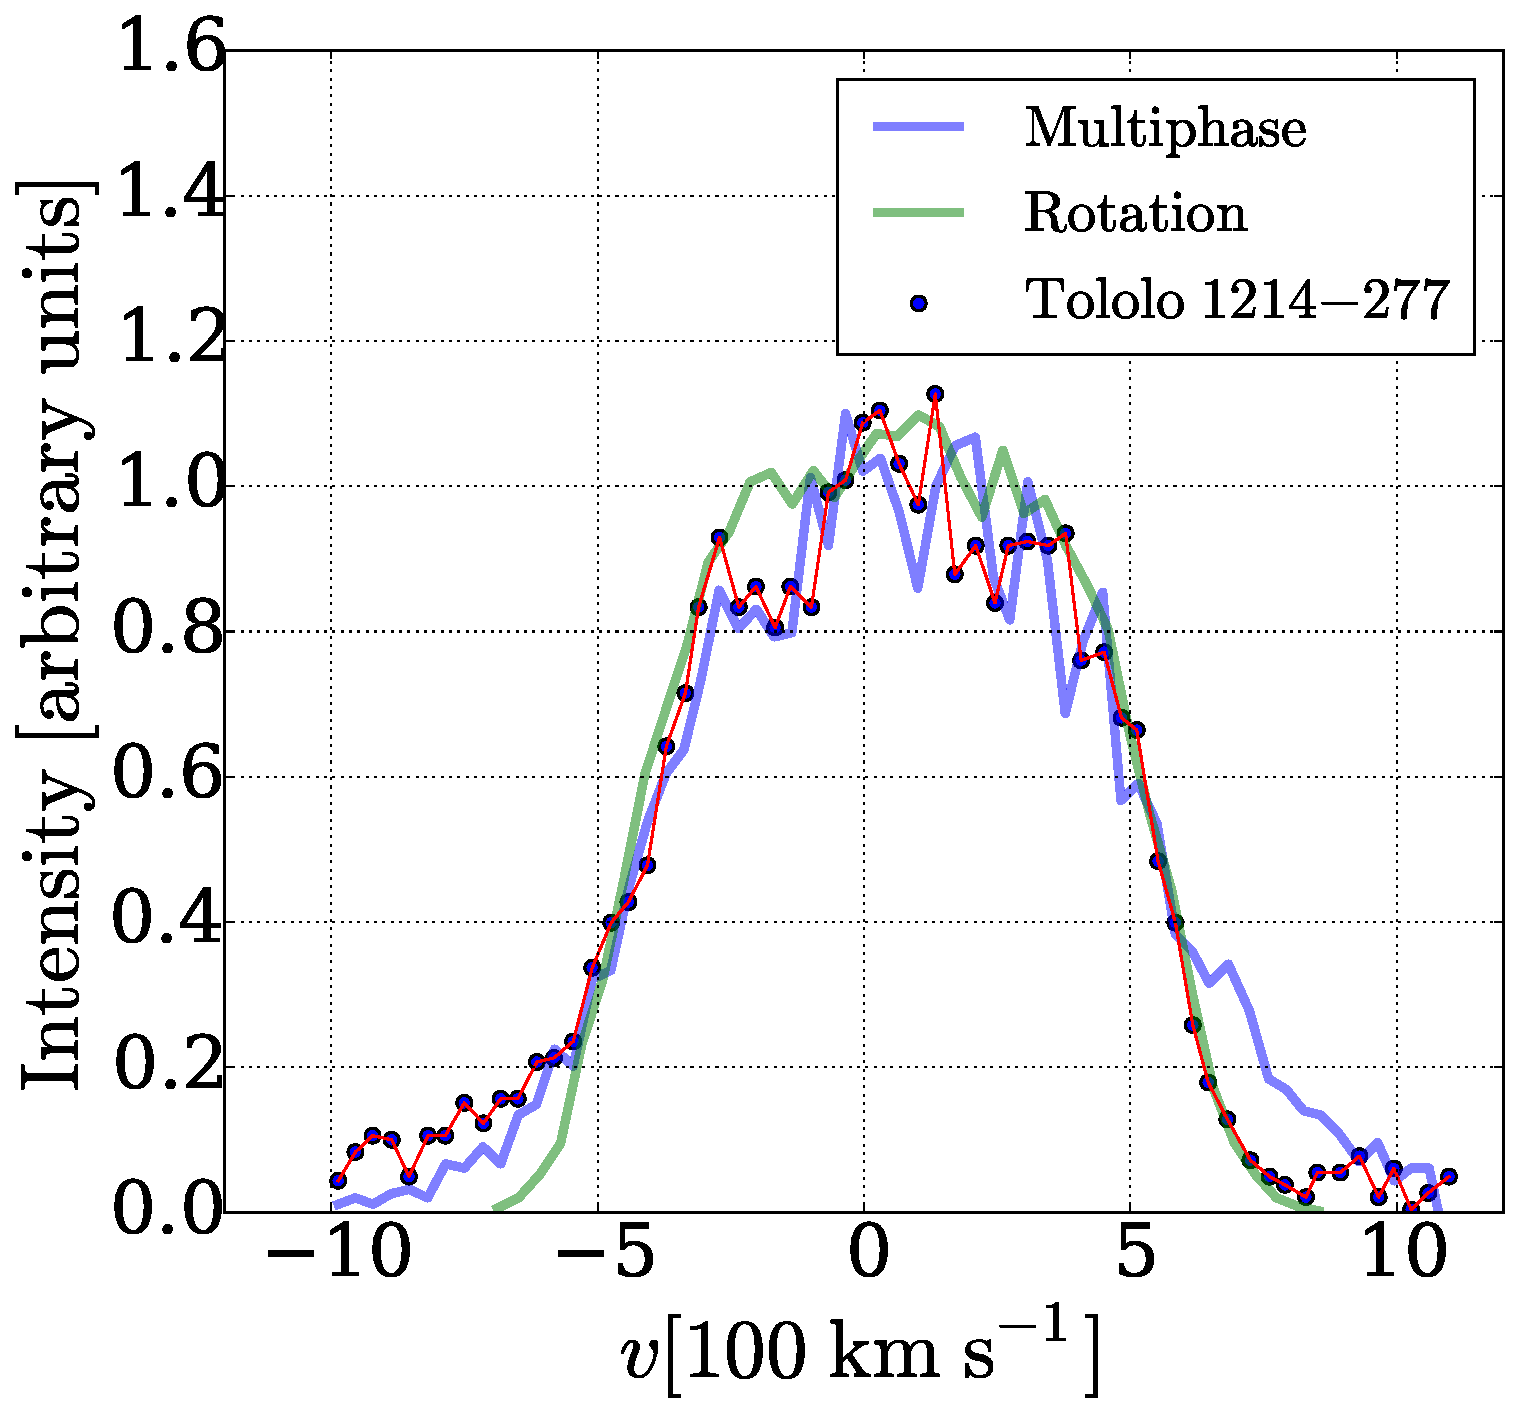
\includegraphics[width=0.55\textwidth]{CLARA-TOL-main.pdf}
\caption{Broad, single peaked and symmetric \lya\ emission of \tol.
  Dots correspond to the observational data \citep{mashesse03}. 
The thick red and thin blue curves represent our best fit
to the data using the full radiative transfer simulation with a
rotation and multiphase model, respectively. 
These two different models are able to reproduce the main morphological
features of \tol's \lya\ line emission.}
\end{center}
\end{figure*}

\begin{figure*}
\begin{center}
  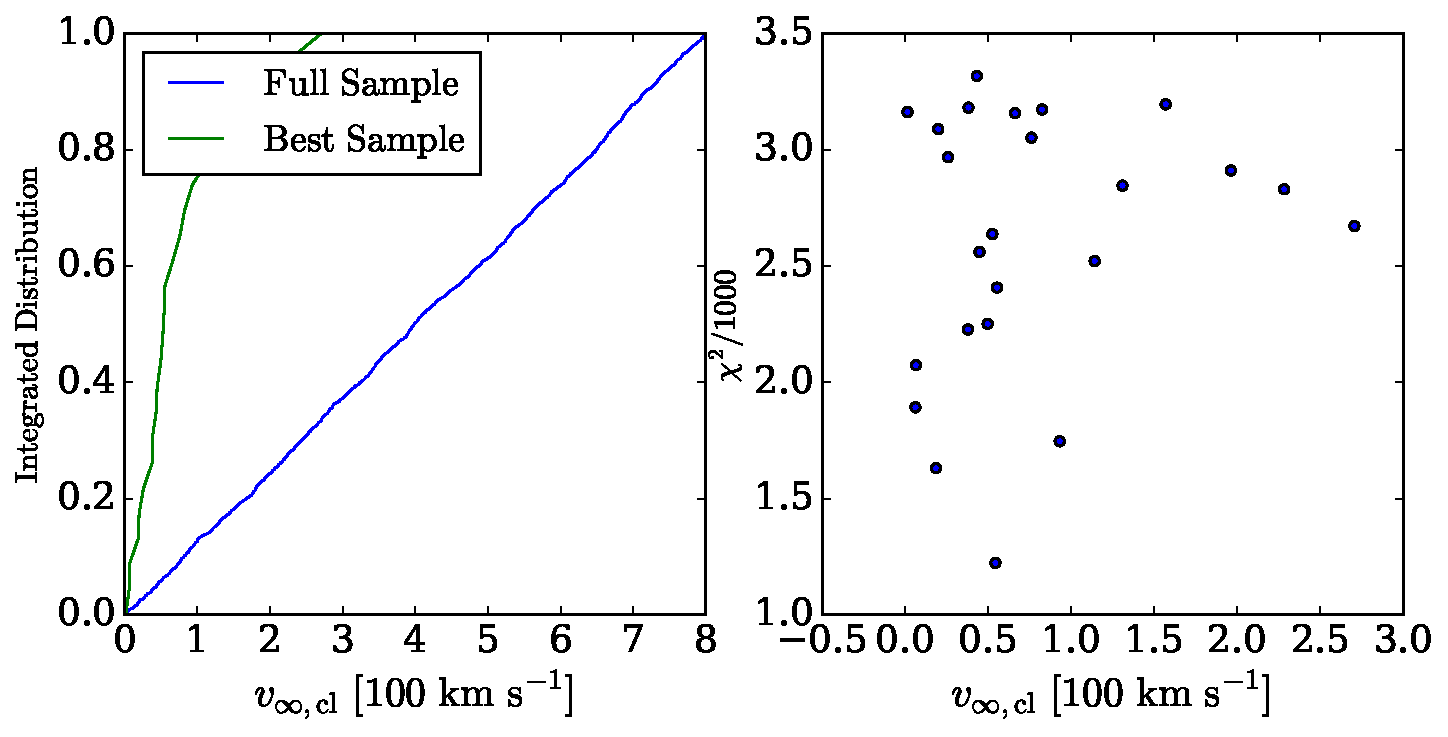
\includegraphics[width=0.6\textwidth]{vinf_cl.pdf}
  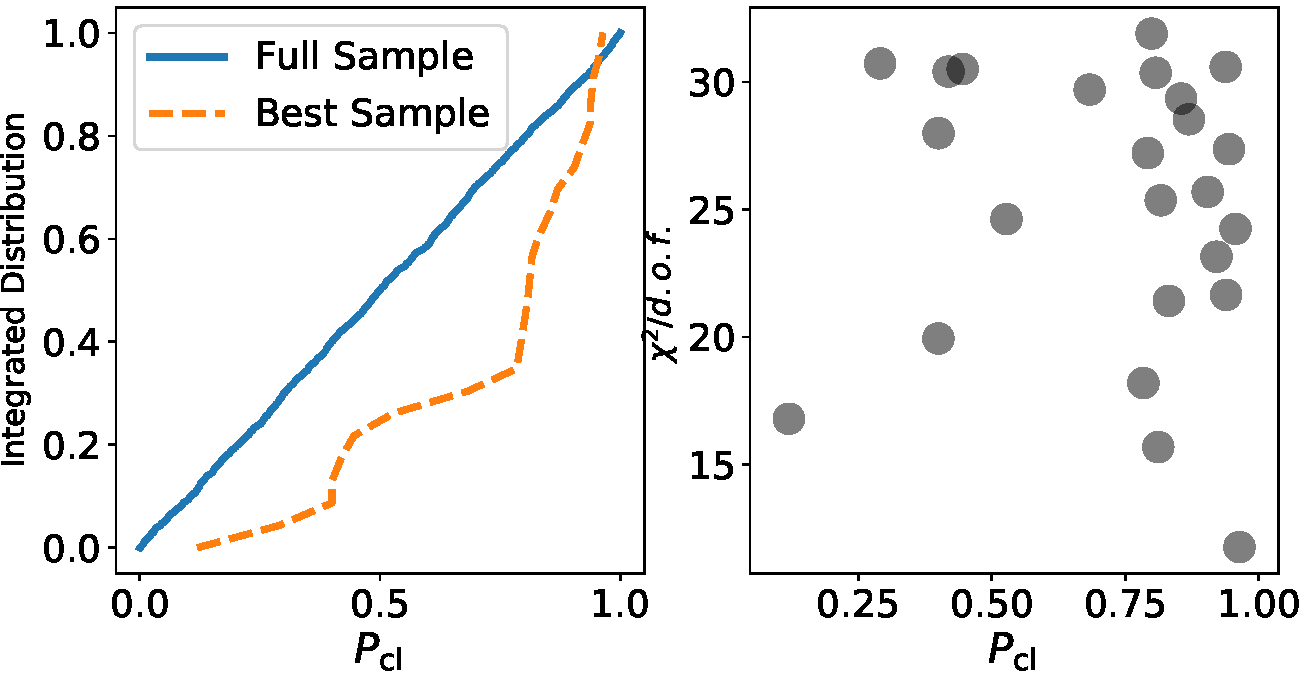
\includegraphics[width=0.6\textwidth]{P_cl.pdf}
  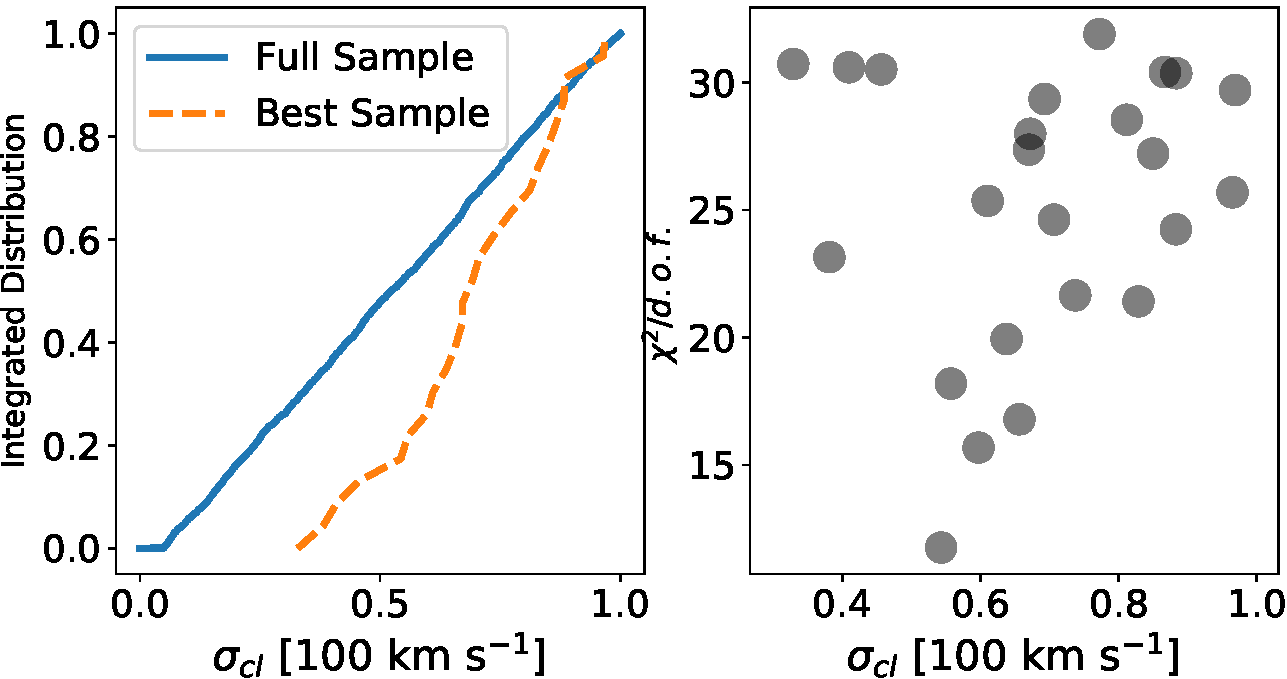
\includegraphics[width=0.6\textwidth]{sigma_cl.pdf}
\caption{Results from the multiphase
  model.
  The left column corresponds to the parameter's integrated distributions for
  models with the lowest $\chi^2$ values (dotted line) compared against the
  parameter's integrated distributions (continuous line) used as a prior.
  These are the only three parameters that show a significant statistical difference from
  the prior distributions, for all the other eleven parameters we
  cannot find any significant difference.
  The right column shows a scatter plot of $\chi^2$ (rescaled by a $1000$)
  and its corresponding physical parameters.
  Only the  25 models with the lowest $\chi^2$ are included.
  \label{multiphaseresults}
}  
\end{center}
\end{figure*}

\begin{figure*}
\begin{center}
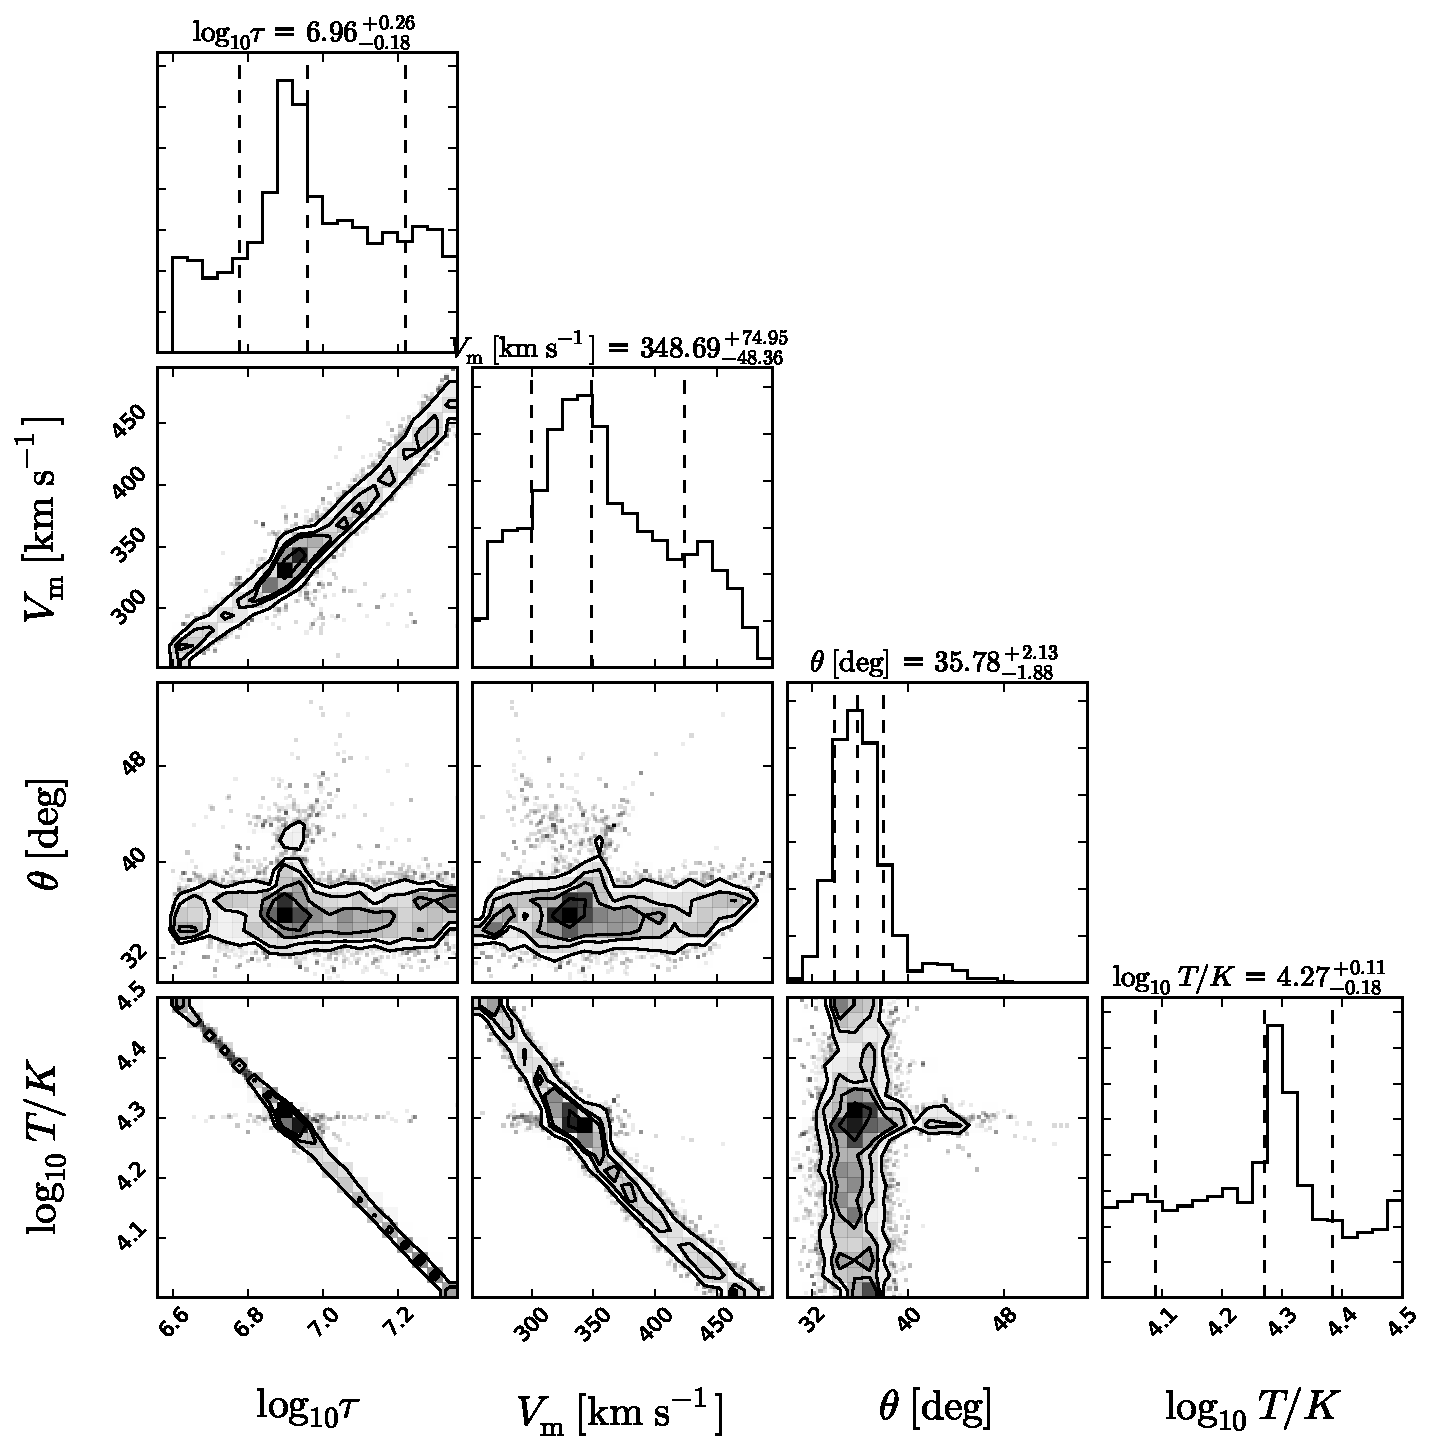
\includegraphics[width=0.8\textwidth]{emcee_results.pdf}
\caption{Results from the Markov Chain Monte Carlo computation for
    the rotation model. The dotted vertical lines in the outer histograms 
	represent the 16th, 50th and 84th percentiles. \label{emceeresults}} 
\end{center}
\end{figure*}


\section{Theoretical Models and Parameter Estimation}


\subsection{Multiphase ISM} 

The idealized multiphase model consists of spherical, cold, dense
clumps of neutral hydrogen (and dust) embedded in a hot, ionized
medium. 
The clumps also have a random and an outflowing velocity
component which totals the number of parameters describing the model
to be $14$, which also include information about the spatial
distribution and thermal state of the clumps and the intraclump
medium. 

In order to map out this large parameter space, we randomly drew
$2500$ sets of parameters within a observationally realistic range,
based on the considerations of \citet{Laursen2013ApJ...766..124L}, 
yielding a large variety of single-, double- and triple-peaked
spectra. 
The full analysis of the the spectral features as well as
more details on the radiative transfer are presented by
\citet{Gronke2016}.    

We compare each resulting spectra to the observational results from
\tol\ after normalizing the observed and simulated spectra to have a 
flux integral of one.
We build a $\chi^2$ on the normalized flux measurements for each one
of the $2500$ models

\begin{equation}
\chi^2 = \sum_{i} \frac{({f}_i - \hat{f}_i)^2}{\sigma_i^2}, 
\label{eq:chi2}
\end{equation}

where $i$ iterates over velocity bins, $f_{i}$ is the observed flux,
$\sigma_i$ is the observed flux uncertainty and $\hat{f}_i$ is the
model estimated flux.
 
We select for further analysis the best $1\%$ models according to the
lowest $\chi^2$ values.
We note that the difference between the lowest and highest $\chi^2$ values in
those $25$ models is close to $\Delta\chi^2 = 3000$, the lowest
$\chi^2$ being close to $\chi^2_{min}=1200$. To have a sense of scale,
the total number of degrees of freedom is $104$. 

Then we perform a Kolmogorov-Smirnov (K-S) test to compare each parameter
distribution in the best $25$ models against the parent distribution
of $2500$ models. 
If we obtain a p-value $<0.05$ for a given model parameter, we conclude that
this parameter does influence the $\chi^2$ fit, as the distribution for
the best $\chi^2$ models is statistically different to the
distribution from the global sample of $2500$ models.  

The best values for the influential parameters correspond to
the values that produce the minimum
$\chi^2$.
We estimate the 1-$\sigma$ uncertainty from a parabolic fit to the
$\chi^2$ as a function of the influential parameters around its
corresponding minimum.   
%$v_{\infty,\rm{cl}}$, $\sigma_{\rm cl}$,
%$P_{\rm cl}$ 



\subsection{Bulk Rotation}

The rotation model corresponds to the work presented in
\citep{GaravitoCamargo2014} based on the Monte Carlo code
\texttt{CLARA} \citep{CLARA}. 
In that model the \lya\ photons are propagated 
within a spherical and homogeneous cloud of HI gas undergoing solid
body rotation.
The sphere is fully characterized by three parameters: the HI line's
center optical  depth $\tau$ measured from the center to its surface, the HI
temperature $T$, and the linear surface velocity $V_{\rm max}$.  
In this model, dust only changes the overall line
normalization and only weakly its shape, i.e. 
dust cannot change the line symmetry or induce a change in the number
of line peaks, moreover it does not change the line width by more than
$1\%$ ($5$ \kms\ in the case of \tol), an effect too small to be
observed at the resolution at which we have \tol's line profile and
also negligeable compared to the influence of the other free parameters in the model.
For these reasons we do not include any dust model. 

We use an analytical solution that captures the most important
effects of rotation onto the \lya\ line as explained by
\citet{GaravitoCamargo2014} and allows us to fully explore the
parameter space using a Markov Chain Monte Carlo (MCMC) calculation with the
\texttt{emcee} Python library \citep{2013PASP..125..306F}. \texttt{emcee} 
is an open source optimized implementation of the affine-invariant 
MCMC sampler \citep{goodman2010ensemble}. 
The algorithm creates a number of walkers that,
during a sufficient number of steps, generate parameters' combinations
for a specific model.
For each timestep, the code calculates the likelihood of the
combination with respect to the observational data.
The walkers explore the parameter space sampling the Gaussian likelihood
function built as $\propto \exp(-\chi^2/2)$, where the $\chi^2$ follows
the definition in Equation \ref{eq:chi2}. 
 

We explore flat priors on four parameters: $200<V_{\rm
  max}/\mathrm{km\ s}^{-1} <600$,   $6.0<\log_{10}\tau<9.0$,
$4.0<\log_{10} T/10^4\mathrm{K}< 4.5$ and $0<\theta<90$ using $500$
steps with $24$ walkers for a total of $12000$ points in the chain.
Previous exploratory work shows that it is impossible to fit the
observed line outside these priors.
Finally, we estimate the parameter values from the 16th, 50th and 84th
percentiles. 


\section{Results}


Figure 1. summarizes our main finding.
Dots represent the observational data for \tol\ with the
overplot from our best fits from the analytical solution for the
multiphase model (thick line)  and the rotating homogeneous gas sphere
(thin line). 

In spite of the simplicity of our models, this is the first time that
the main \tol\ features can be reproduced: a wide, centered,
single-peaked \lya\ line.
This result does not demonstrate that the kinematic features we
include in our models are necessary to reproduce \tol's features, but
at least they show that they are a sufficient condition.
This is a significant step forward to understand the influence that
different kinematics have in producing the atypical line profile shown
by \tol.

In what follows we summarize the values of the kinematic parameters
that managed to explain \tol\'s \lya\ profile.


\subsection{Multiphase ISM}

From the K-S tests we find that only three parameters can be
constrained by the observations: the clump outflow velocity
$v_{\infty,\rm{cl}}$ (p-value  $10^{-18}$), the clump velocity
dispersion $\sigma_{\rm cl}$ (p-value $10^{-4}$) and the probability
that the \lya\ emission comes from the clumps $P_{\rm cl}$ (p-value
$10^{-4}$).
This does not mean the other parameters do not influence the resulting
spectra at all; it means that they cannot be constrained from \tol's
observations.


The results are summarized in Figure \ref{multiphaseresults}.
Left panels show the difference between the integrated distributions
of the full sample (2500 input models) and the models with the lowest
$\chi^2$. 
The right panel shows the actual $\chi^2$ values and its corresponding
parameter value. 
Under these conditions we find $\sigma_{\rm cl}=$\sigmaclump,
$v_{\infty {\rm, cl}}=$\inftyclump\ and $P_{\rm cl}=$\probaclump. 

Qualitatively, as \tol\ possesses a very wide spectrum which can be
achieved by subsequent scatterings off (relatively) fast moving clumps
while the multi-phase nature (i.e., the existence of low-density
channels) ensures the high flux at line center as observed.
In turn, a lower velocity dispersion would produce a thiner line than the
observed.
From the lower right panel in \ref{multiphaseresults} we find that it
is unlikely that the clump velocity dispersion is lower than
$50$\kms. 

Why is it that the other parameters do not seem to matter? Probably
because $P_{cl}$ (the probability for a \lya\ to be emitted in a
clump) is high and most photons are produced at
large radii making the radiative transfer effects in the center less
important.  
We cannot discard that another region of parameter space with similar
velocity structure but empty interclump medium, relatively dense
clumps and at least a few clumps per sightline 
could also work \citep{Hansen06}.
This possibility does not change our conclusions about the
kinematic parameters, but it might be interesting to explore in the
future with a higher sampling of the parameter space once new
observations clarify the kinematic nature of \tol.  

\subsection{Bulk Rotation}


The results are summarized in  Figure \ref{emceeresults}. 
From this analysis we find that the best parameters in the rotation
model are a rotational velocity of  $V_{\rm max}=348^{+75}_{-48}$
\kms, a neutral Hydrogen optical depth of
$\log_{10}\tau=6.96^{+0.26}_{-0.18}$,  and an inter-stellar medium
temperature of $\log_{10} T/\mathrm {K} = 4.27^{+0.11}_{-0.18}$.   
This model is also able to constrain the angle between the plane
perpendicular to the rotation axis and the observational line-of-sight
to $\theta = 35.78^{+2.13}_{-1.88}$ degrees.

Lower rotational velocities are disfavored by the fact that the line
is single peaked.
Fixing the optical depth at a high value of $10^7$ ensures that the line width
is close to its observed value.
A lower rotational velocity would produce a double peaked line.
The fact that the velocity and optical depth priors were wide enough,
allows us to think that the current values found by the MCMC are
robust given the observational constraints.




\section{Discussion}

\tol\ shows one of the most atypical \lya\ spectra observed so far.
Its flux at the line's center is high compared to other LAEs at low
redshift and the wide symmetrical peak is virtually absent from other
LAEs at low and high redshift \citep{LARS,Erb14,Trainor16}. Simple
shell models fail to reproduce such a spectrum
\cite{2015A&A...578A...7V}.  
In the previous sections we show how these characteristics can be
explained by rather extreme kinematic characteristics.
Now we discuss and frame those results in terms of the dynamical mass
that could explain the velocities obtained in the model.

Using the constraints for the velocity dispersion $\sigma$ and the
maximum rotational velocity $V_m$ in a spherical system localized in a
region of size $r$ we can estimate two different values for the
dynamical mass within $r$: 

\begin{equation}
M_{\rm dyn} = 3 \frac{\sigma ^{2}r}{G} = 3.48\times10^{9}
\left(\frac{\sigma}{100\ \mathrm{km\ s}^{-1}}\right)^2\left(\frac{r}{\mathrm{kpc}}\right)
M_{\odot}, 
\end{equation}
%
and
%
\begin{equation}
M_{\rm dyn} = \frac{V_m ^{2}r}{G} = 1.16\times10^{9}
\left(\frac{V_m}{100\ \mathrm{km\ s}^{-1}}\right)^2\left(\frac{r}{\mathrm{kpc}}\right)M_{\odot}, 
\end{equation}
%
for the multiphase and rotation model, respectively.
Assuming that the \lya\ emission is entirely powered by star formation 
we use the 3D half-light radius $r_s=2.25$ kpc as the typical size
for the HI region,


In the multiphase model the clump velocity dispersion
$\sigma_{\rm{cl}}=$\sigmaclump corresponds to a dynamical mass of
$M_{\rm dyn}=2.31\pm0.04 \times 10^{9}$ $M_{\odot}$, while the
rotational velocity of $V_{\rm max}=348^{+75}_{-48}$\kms corresponds
$M_{\rm dyn} = 3.2_{-1.0}^{+1.6}\times 10^{10} M_{\odot}$.


\tol's stellar mass is  $M_{\star} = 1.45\pm0.45\times 10^{8}
M_{\odot}$   \citep{2014PASP..126.1079M} and its total neutral HI mass
is $M_{\rm HI}<2.65\times 10^{8}$ M$_{\odot}$ 
\citep{pustilnikmartin07}; the dynamical mass is at least 12 to 160 times
the baryonic mass, depending if one considers the multiphase or
bulk rotation estimate. 
We lean towards the lower dynamical mass estimate from the multiphase
model as it seems easier to reconcile with the following two
astrophysical mechanisms for its origin.

A first possibility to explain a dynamical mass of $10^{9} M_{\odot}$
in a sphere of 2.25 kpc in radius, could be a dark matter halo of at
least $10^{12}$ M$_{\odot}$ in mass \citep{2011ApJ...726..108T}.
This estimate is based on computing the integrated mass profile of a
spherical dark matter halo with a Navarro-Frenk-White profile with its
concentration following the \emph{median} mass-concentration
relationship found in the Bolshoi simulation
\citep{2012MNRAS.423.3018P}. 
This estimate leaves open the question as to why  \tol\ is not more
similar to the Milky Way galaxy as it would be hosted by a dark matter
halo of similar mass.

A second possibility is that \tol\ hosts a supermassive black hole of
$10^{9} M_{\odot}$. This is almost two orders of magnitude higher
than the supermassive black hole found in the compact dwarf galaxy
M60-UCD1 \citep{2014Natur.513..398S}, which has a similar stellar mass
as \tol. This would leave open the question about the formation
process of such a system.   

%Another perspective to appreciate the atypically high dynamical mass
%estimates comes from the observed scaling relations for dwarf
%galaxies.
%Assuming that \tol\ followed the fundamental plane relationship
%between its mean surface brightness $I_e$, the projected half-light
%radius $R_e$ and the velocity dispersion $\sigma$, described by $\log
%I_e=1.6 \log\sigma - 1.21\log R_e + 0.55$ \citep{2009ApJ...698.1590G},
%the expected velocity dispersion should be on the order of $5 \pm 1$ 
%\kms, which is a factor of $\sim$ $10$ - $60$ lower than the 
%results from the multiphase and rotation models, respectively. 
%These are equivalent to factors of $\sim$ $100$ - $3600$ on the
%dynamical mass.
%Once again,  \tol\ seems to be significantly more massive than
%expected. 

A new observational test is needed to clarify the kinematic nature of
\tol. 
We suggest that integral field unit measurements 
resolving its spatial extent are up to the task. 
\tol\ spans a region of $4$ arcseconds,
an instrument such as the Multi Unit Spectroscopic Explorer (MUSE)
\citep{2014Msngr.157...13B} with its
nominal $0.2$ arcseconds spatial sampling over a $1.0$ arcminute field
in wide-field mode could provide a coarse mapping of different
ionization lines to infer a kinematic map in the H$\alpha$ line,
following the kind of work presented by \citet{Herenz16} done with the Potsdam
Multi-Aperture Spectrometer (PMAS) \citet{PMAS} on nearby
\lya\ emitting galaxies.
We note that archival Chandra X-ray archival
data \footnote{\url{http://cxc.harvard.edu/cda/}} does not show any
detection for \tol.
This lack of detection would also put an upper limit on the intensity
of recent black hole activity due to accretion. 

Another observational test includes the measurement of the
\lya\ ionizing continuum escape fraction.
In the rotational model this fraction should be zero, while
the multiphase model predicts that averaging over all sightlines
it should be around $0.5^{+1.0}_{-0.4}$\%, with the possibility of strong
variations depending on viewing angle (i.e. some sightlines can have
an escape fraction close to $100\%$)\citep{Gronke2016} . 



\section{Conclusions}

In this paper we presented two kinematic models that independently
reproduce the so far unexplained observational features of \tol's
\lya\ emission line.  One model is based on a multiphase ISM with random clump motions and
the other on gas bulk solid body rotation.

It is the first time that an observed \lya\ profile can be fully
reproduced by either of these two kinematic conditions.
Furthermore, the kinematics of both models suggest a dynamical mass
at least ten times larger than the baryonic mass infered from observations.
We suggest that additional integral field unit observations are the
only way to be certain about the detailed kinematic structure in \tol.

All in all, the mere existence of a strong LAE galaxy with a broad,
symmetric line is interesting. 
\tol's line shape is different to others and reveals an unexpected
kinematic structure.
Our findings highlight the importance of including multiphase and/or
rotation conditions as kinematic features to model the \lya\ line.

Additionally, if the hypothesis of a supermassive black
hole in \tol\ proves to be consistent with future observational
kinematic maps, it could correspond to a so far undetected
supermassive black hole in a dwarf galaxy, providing a new way to test
and probe theories on the co-evolution of galaxies and black holes in
the first generation of galaxies.   

\section*{Acknowledgments}
We thank J. M. Mas-Hesse for providing us with \tol's observational
\lya\ data \citep{mashesse03} in electronic format. This data was
used to prepare Figure 1.



\bibliographystyle{mn2e}
\bibliography{references}


\end{document}

